\section{Flip-Flop D \label{sec:s3}}

\begin{center}
	\begin{minipage}{12cm}
		\begin{tcolorbox}[title=Actividad 3]
			 Un flip-flop D puede construirse a partir de dos latch tipo D en cascada (configuración MASTER-SLAVE) de acuerdo al siguiente diagrama:
			 \begin{figure}[ht]
			 	\centering
			 	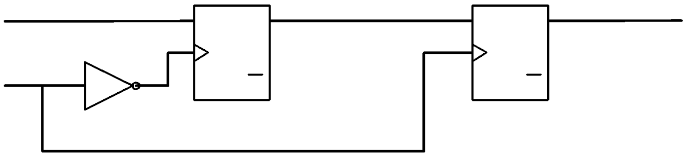
\includegraphics[scale=0.5]{FlipFlopD.png}
			 \end{figure}
			 Usar dos instancias del latch D del inciso 2. Repetir los pasos del inciso 1.
		\end{tcolorbox}	
	\end{minipage}
\end{center}

e